\documentclass{article}
\usepackage{amsmath,amsfonts,amsthm,fullpage}
\usepackage{algorithm}
\usepackage{algorithmic}
\usepackage{graphicx}
\usepackage{hyperref}

\begin{document}
\title{ISYE 6740 Summer 2023 Project Report 

``Augmented recipe recommendation using flavor profile, ingredients, and cooking technique''}
\author{Micaela McCall}
\date{July 29 2023}
\maketitle

\tableofcontents
\pagebreak

\section{Background and Literature Review}

As the amount of information on the internet has ballooned, recommendation systems have become increasingly crucial to help users find desired information without having to do extensive manual search. The goal of a recommender system is to predict the rating a user would give to a new item and to suggest to the user items for which the predicted rating is high. Food and recipe recommendation is a domain in which these systems are particularly relevant given the vast number of online recipes. Recipe recommendation has gained traction in the healthy-eating community as a way to suggest healthier meals or ingredient substitutions [1, 2, 3]. It is also a relevant context for group recommender system research; i.e., how to suggest recipes based on the preferences of all members of a group [4]. %Another relevant sub-domain of recipe recommendation is in the area of sustainability. This means recommending recipes based on measures of sustainability, such as food miles, rather than just user preferences. 
\vspace{0.1in}
\\
In addition to its many applications, basic recipe recommendation  offers fertile ground for researching the nuances of recommendation systems because of the rich information about recipe contents (ingredients), types of recipes (breakfast, dinner, desert, etc.), styles of cooking, nutritional contents, etc.  Some relevant questions in this area are: How do we quantify a user's preference for specific ingredients given their rating of a recipe and leverage this information to improve recommendation? How do we incorporate preferences for particular types of recipes? How do we build recommender systems under constraint, such as only recommending recipes that conform to dietary restrictions?
\vspace{0.1in}
\\
Researchers have tried to address some of these questions through iteration on various approaches to algorithmic recommendation. Some of the most common are: 
\vspace{0.1in}

\textbf{Collaborative filtering (CF)} is a method that uses the ratings of many users over many items to identify similar users and predict the rating a user would give to an item based on the ratings given by similar users. The only data necessary for this approach is ratings history on items [5].
\vspace{0.1in}

\textbf{Content-based (CB)} is a method that uses information about items to calculate similarity between new items and items a user has historically rated to predict the rating a user would give to an item [1]. For example, in the recipe/food domain, Freyne and Berkovsky (2010) broke down ratings for a recipe into ratings for ingredients and then reconstructed a prediction for a new recipe using a user's ratings for the constituent ingredients.
\vspace{0.1in}

\textbf{Knowledge-based (KB)} is a method that uses content knowledge about the item as well as knowledge about users needs or a set of constraints to recommend specific items and then includes an iterative process of eliciting users' feedback. [1, 7] 
\vspace{0.1in}

\textbf{Hybrid approaches} are particularly used in recipe recommendation because we have both plentiful user ratings data and about item content. These approaches aim to combine the strengths of multiple previously mentioned approaches. [1, 7]
\vspace{0.1in}
\\
In my literature review, I noticed that many attempts to recommend healthy foods used a KB approach; they didn't just reflect the user's preferences, but also the nutritional needs of the particular user based on their demographic information, e.g. in Alberg (2006). Attempts to conform to dietary restrictions were treated similarly [8]. However, I didn't find instances where rich recipe-based metadata was included in recommender algorithms to try to improve the quality of the recommendation, other than in Freyne and Berkovsky (2010). 

\section{Problem Statement}
The aim of this project is to explore and compare the performance of CB, CF, and hybrid recommender algorithms in the context of recipe recommendation, while leveraging recipe flavor profiles and recipe metadata (meal type, cooking technique, cooking time) in the recommendation.
\vspace{0.1in}
\\
In contrast with some of the approaches mentioned above, I didn't search for access to a data set where recipe ratings for individuals with rich person-centered metadata was available. Rather, my goal is to use solely recipe-related metadata, and enhance this with a second data source of flavor profiles, directly in the implementations of CB, CF, and hybrid recommender algorithms. 
\vspace{0.1in}
\\
Additionally, in the context of CB recommendations, I want to expand on the approach used by Freyne and Berkovsky (2010) to include recipe flavor and metadata. 

\section{Data Sources}

The first data set is a set of recipes from Food.com, made available on as a Kaggle dataset (\url{https://www.kaggle.com/datasets/shuyangli94/food-com-recipes-and-user-interactions?resource=download&select=RAW_recipes.csv}). The recipes data ncludes the name of the recipe, a description of the recipe, recipe tags, the nutritional value, the steps in make the recipe, and the ingredients. 
\vspace{0.1in}
\\
The second data set is a set of recipe interactions also from Food.com and also made available through Kaggle (\url{https://www.kaggle.com/datasets/shuyangli94/food-com-recipes-and-user-interactions?resource=download&select=RAW_interactions.csv}). This data set includes the rating and review given to a recipe by various users (recipe id matches up to the recipe id in the recipes data set above). 
\vspace{0.1in}
\\
The third data set provides the flavor molecules and associated flavor profile for a given food (from \url{https://cosylab.iiitd.edu.in/flavordb/}). It is accessed via API calls for each ingredient in the recipes from the first datset. 
\vspace{0.1in}
\\
A final data set provides ingredient lemmatization, or in orther words associating each possible ingredient with a "base" version of that ingredient (e.g. all types of lettuce become "lettuce"). Also made available through Kaggle (\url{https://www.kaggle.com/datasets/shuyangli94/food-com-recipes-and-user-interactions/discussion/118716?resource=download&select=ingr_map.pkl}).

\section{Methodology}

\subsection{Data gathering}

A unified list of ingredients was collected for all recipes in the following way: for each recipe, I applied a SpaCy model to a string representation of its ingredients and only the noun and proper nouns were preserved, and then all noun and proper nouns were given a unique id and added to a de-duplicated list. The reason for this pre-processing step is that each word in the list was queried in the FlavorDB API, and it wouldn't do to query a modifier (e.g. ``fresh" in the ingredient ``fresh strawberries"). 

For each ingredient in this list, I queried the FlavorDB search API to find the most similar search result that exists in their DB. For the search match, the search term was then used in the query for specific flavor molecules, which were subsequently matched with their individual flavors. This resulted in many flavors for each particular ingredient as per this example.

\begin{figure}[h]
    \centering
    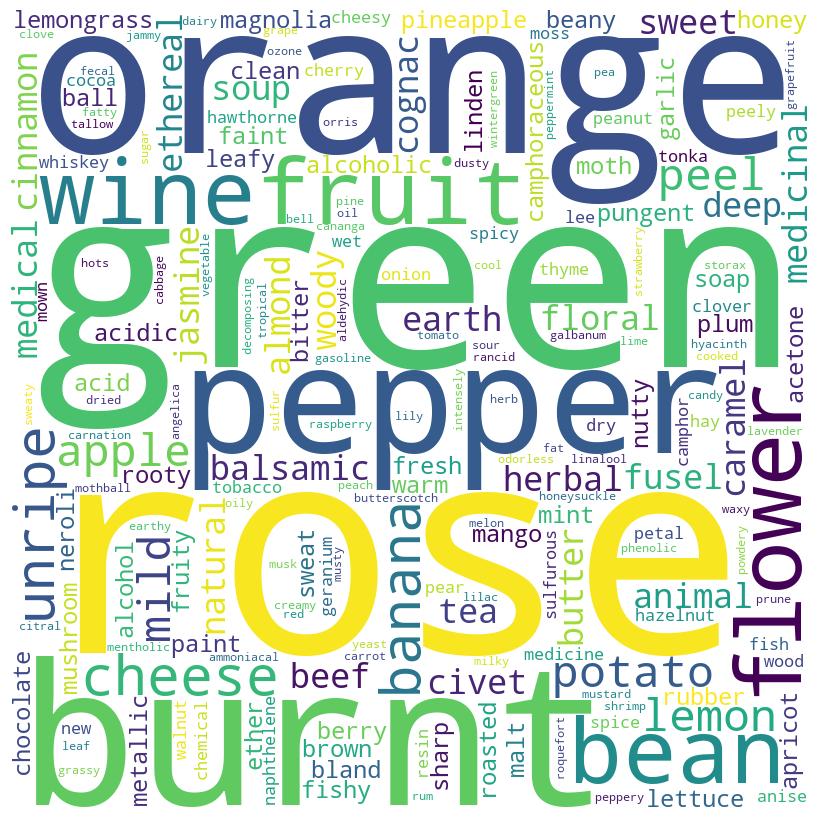
\includegraphics[width=0.5\textwidth]{lettuce_word_cloud.png}
    \caption{The flavors associated with the ingredient ``lettuce"}
    \label{fig:lettuce_word_cloud}
\end{figure}


\subsection{Data Preprocessing}

Each recipe id was merged with its constituent ingredients and each ingredient's' corresponding flavors. In addition, the data set was downloaded with a set of technique ids associated with each recipe. After tracking down the corresponding techniques in the following source code for the data set, I was able to match each technique to each recipe that used it. At this point, each recipe ``detail" was collated and given a detail id (ingredients, flavors, and techniques). 

These data were merged with the user interactions data such that the rating for each recipe could also be associated with each detail of that recipe. For example, when averaging the rating across all the recipes that has a particular ingredient, you would get the average rating for that ingredient across the whole data set. \begin{figure}[H]
    \centering
    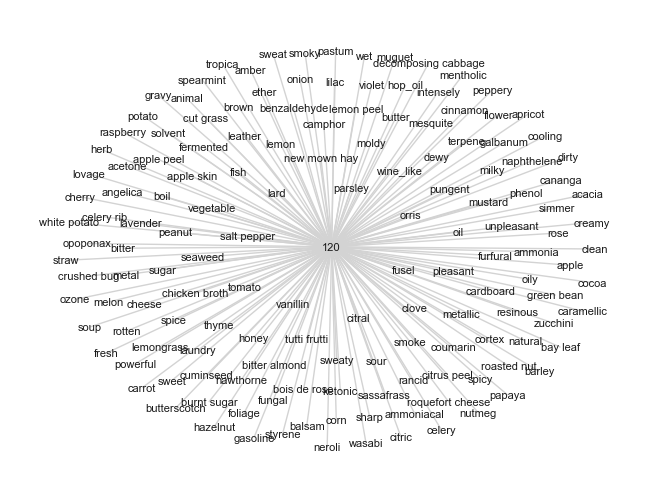
\includegraphics[width=0.8\textwidth]{flavs120.png}
    \caption{Some of the details associated with Recipe 120}
    \label{fig:flavs120}
\end{figure}

\begin{figure}[H]
    \centering
    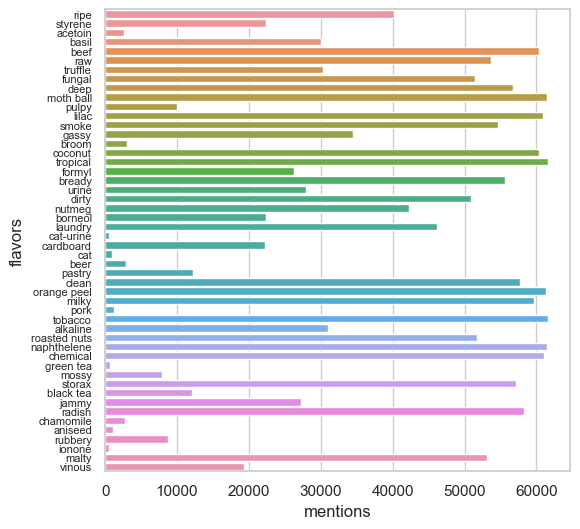
\includegraphics[width=0.6\textwidth]{flavors_mentions.png}
    \caption{Some of the flavors and their number of mentions across the data set}
    \label{fig:flavors_mentions}
\end{figure}

\begin{figure}[H]
    \centering
    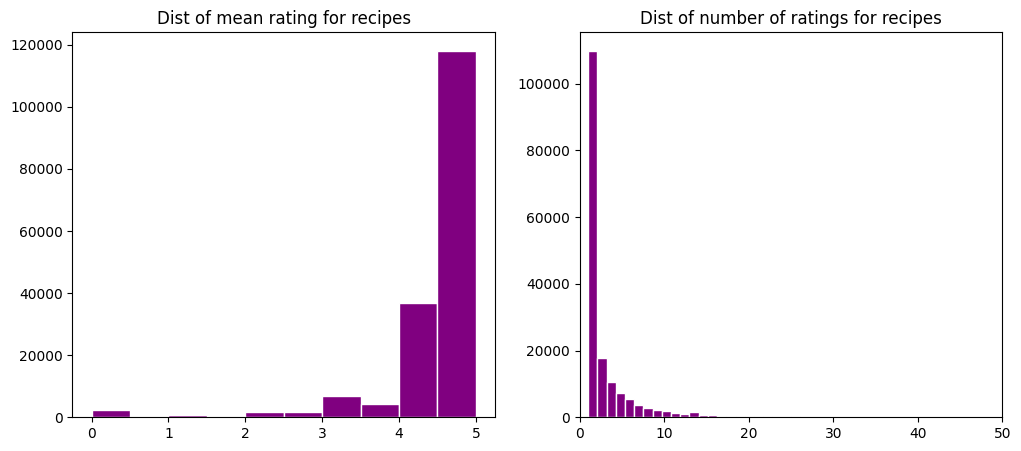
\includegraphics[width=0.9\textwidth]{ratings_dist.png}
    \caption{Distribution of average and count of recipe rating}
    \label{fig:ratings_dist}
\end{figure}


\subsection{Train-test split}

I created my training and testing sets in an intentional way because I wanted to make sure that I could generate ratings for as many user-recipe pairs as possible. Namely, for each recipe where there was at least 10 ratings, I randomly selected one user-rating for that recipe to be part of the test set. This guaranteed that I wouldn't run into the issue when testing that data that a recipe in the test set does not exist at all in the training set. Now, it's still possible that there could not exist a rating for a recipe among the closest neighbors of a particular user, so this doesn't entirely fix the possibility that I may not be able to generate predictions for some user-recipe pairs. 


\subsection{Recommendation Algorithms}

Each of the following algorithms was applied on the recipe interactions data. 
\vspace{0.1in}
\\
\textbf{Baseline model}

First, built a model that randomly predicts ratings for a given user on a given recipe by sampling from a uniform distribution. 
\vspace{0.1in}
\\
\textbf{Collaborative filtering (CF)}
\vspace{0.1in}

\textbf{Nearest neighbors:} calculate the nearest neighbors of a new user measured by cosine similarity:
\begin{equation}
    Sim(u_i, u_k) := \frac{r_i * r_k}{||r_i||*||r_k||} = \frac{\sum_{j=1}^mr_{ij}r_{kj}}{\sqrt{\sum_{j=1}^mr_{ij}^2\sum_{j=1}^mr_{kj}^2}}
\end{equation} where $r_i$ and $r_k$ are ratings vectors for users $u_i$ and $u_k$. 

Predict a user's rating on a new recipe $r_{ij}$ by weighted average with bias avoided by by subtracting each user's average rating $\tilde{r_k}$ from their rating of the recipe and adding in the target user's average rating $\tilde{r_i}$:
\begin{equation}
    r_{ij} = \tilde{r_i}+\frac{\sum_kSim(u_i, u_k)(r_{kj}-\tilde{r}_k)}{\text{num ratings}}
\end{equation}
\vspace{0.1in}

\textbf{Matrix Factorization:} aims to decompose the user's preferences for into preferences for a set of latent factors. Matrix factorization can be performed using Singular Value Decomposition (SVD): 
\begin{equation}
   M = U\Sigma V^T
\end{equation} By selecting the top $k$ singular values of matrix $\Sigma$, we can reconstruct matrix $M$ with less dimensions but still capturing much of the variability of the original matrix [9]. The concept here, when applied over recipe ratings, would be to find the dimensions of latent food preferences so as to avoid having to deal with the high dimensionality of individual recipe ratings.

However, when factoring a sparse matrix, it's more efficient to use Non-negative Matrix Factorization (NMF), which involves finding  $P$ and $Q$ such that the reconstructed user-item rating $\hat{r}_{ui}= q_i^Tp_u$ is as close as possible to the true ${r}_{ui}$. In order to find $P$ and $Q$, the Mean Squared Error is minimized:

\begin{equation}
   min_{q,p} \sum_{(u, i) \in TR} (r_{ui} - q_i^Tp_u)^2 + \lambda(||q_i||^2+||p_u||^2)
\end{equation} where $p_u$ is the user vector, the $u$-th row of matrix $P$, and $q_i$ is the item vector, the $i$-th row of matrix $Q$, and $TR$ is the training set [9]. I implemented this optimization by hand by performing Gradient Decent according to the implementation in Luo et al. (2014). On each update of the Gradient Decent, the entries of the $P$ and $Q$ matrices are updated as below:

\begin{equation}
   p_{u,k} \leftarrow p_{u,k}\frac{\sum_{i \in TR}q_{k,i} r_{u,i}}{|I_u|\lambda p_{u,k} + \sum_{i \in TR} \hat r_{u,i}}
\end{equation}

\begin{equation}
    q_{k,i} \leftarrow q_{k,i}\frac{\sum_{i \in TR}p_{u,k} r_{u,i}}{|U_i|\lambda q_{k,i} + \sum_{i \in TR} \hat r_{u,i}}
\end{equation} where $I_u$ is the number of ratings for that user in the item set, and $U_i$ is the number of rating for that item in the user set. A prediction for a new user-recipe pair is simply the $\hat r_{ui}$ entry in the reconstructed $\hat R = PQ^T$ matrix.
\vspace{0.1in}
\\
\textbf{Content-based (CB)} 

A rating for each user on each ingredient is calculated as the average of the ratings each user gave to all recipes including that ingredient:
\begin{equation}
    rat(u_i, ingr_j) = \frac{\sum_{l; ingr_j \in l}r_{il}}{l}
\end{equation} where $r_{il}$ is the rating user $i$ gave to recipe $l$.
This formula is then applied over the flavor profile of each recipe, tags, and cooking techniques, to create a comprehensive recipe-based data source for each user. 
Predict a user's rating on a new recipe $r_{ij}$ by finding the average rating across all the ingredients, flavors, and cooking techniques in the new recipe:
\begin{equation}
    r_{ij} = \frac{\sum_{l\in rec_j} rat(u_i, ingr_l)}{l}
\end{equation}
\vspace{0.1in}
\\
\textbf{Hybrid} 

\vspace{0.1in}
\textbf{Content-augmented CF using cosine similarity}: attempts to generate as many ratings as possible for a user on ingredients, flavors, and techniques using ratings given by similar users, and then uses an average of the ratings of the content of a recipe to predict a new user-recipe rating. 
\\
To be more specific, this involved three steps:

\textbf{1. }  I used Equation 1 to find the nearest neighbors of a new user (as in the CF approach).

\textbf{2.} Then, I used the following equation to predict a new user's ratings on ingredients, flavors, and techniques that they hadn't already rated:

\begin{equation}
    rat(u_i, ingr_d) = \frac{\sum_k Sim(u_i, u_k)rat(u_k, ingr_d)}{\text{num ratings of }d}
\end{equation}

\textbf{3.} Then I used Equation 8 to predict a user's rating on a new recipe $r_{ij}$.

\vspace{0.1in}
\textbf{Content-augmented matrix factorization}: takes the matrix factorization approach to CF and augments the item data with content. I used NMF for this approach, like the basic matrix factorization approach. However, I incorporated recipe content information into this factorization by further factoring the matrix $Q$ (shape: num features by num recipes) as $X\Phi$, where $X$ is a matrix (shape: num recipes by num ingredients) in which $X_{id}$ is a binary indicator if ingredient $d$ is in recipe $i$. This results in the following NMF factorization of matrix $R$:
\begin{equation}
    R = P\Phi^TX^T
\end{equation} My source for this approach is Forbes et al. (2011). This updated NMF results in the following minimization of MSE:
\begin{equation}
   min_{\phi,p} \sum_{(u,i) \in TR} (r_{ui} - p_u\Phi^Tx_i^T)^2 
\end{equation} 

Rather than implementing the updates to each matrix on each iteration of Gradient Descent by hand like I did for the basic matrix factorization, I decided to use Pytorch to calculate and update the matrices according to MSE loss. Once training is complete, a prediction for a new user-recipe pair is simply the $\hat r_{ui}$ entry in the reconstructed $\hat R = P\Phi^TX^T$ matrix.

\section{Evaluation and Final Results}

I trained each model above using the training set described previously, and then generated predictions using each user-recipe pair in the testing set. I used Root Mean Square Error (RMSE), Mean Absolute Error (MAE) and coverage (ability to generate predictions) [6] to evaluate the performance of each approach. 
\vspace{.1in}

\begin{tabular}{|| p{30mm} | p{15mm} p{15mm} p{15mm}||} 
 \hline
  Model &  RMSE & MAE & Coverage \\ [0.5ex] 
 \hline\hline
 Baseline & 2.5185 & 2.04112 & 1.0 \\
 \hline
 Vanilla CF & 0.9805 & 0.5617 & 1.0 \\
 \hline
 Matrix \newline factorization CF & 1.7859 & 1.4959 &  0.6837\\
 \hline
 CB & 1.3987 & 1.0338 & 0.3343 \\
 \hline
 Content-augmented CF & 1.0787 & 0.8480 & 0.9995 \\
 \hline
 Content-augmented  matrix \newline factorization &  4.1741 &  3.8136 &  1.1\\
 \hline
\end{tabular}

\vspace{.1in}

Below are further details on the implementation and results of each algorithm. I found that plotting the rating predictions across the true ratings in the test set was a helpful way to see differences in trends across different algorithms. 

Because this data set is very skewed, specifically in that there are many more ratings of 5 and 6 then 1, 2, and 3, this results in some issues with the metrics mentioned above, namely that by predicting a score of 6 across all ratings, you can actually get fairly good metrics. We can see below that that is what happened with the several of the models. 

\subsection {Baseline model}

As mentioned in section 4.4, these predictions were selected from a uniform random distribution betwen 1 and 6. 

\begin{figure}[H]
    \centering
    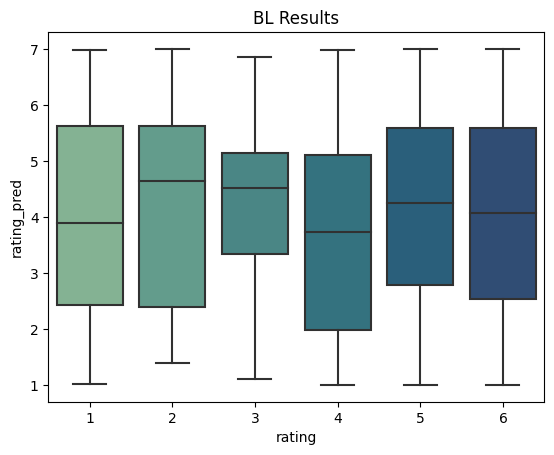
\includegraphics[width=0.6\textwidth]{BL.png}
    \caption{Distribution of predicted ratings across true ratings for baseline algorithm}
    \label{BL}
\end{figure}

\subsection{Vanilla CF model}

For this model, I compared results for the most similar 10 users, most similar 50 users, and most similar 100 users. 

Below are the predictions results of averaging the ratings of the most similar 50 users for each user-recipe pair in the test set. 

\begin{figure}[H]
    \centering
    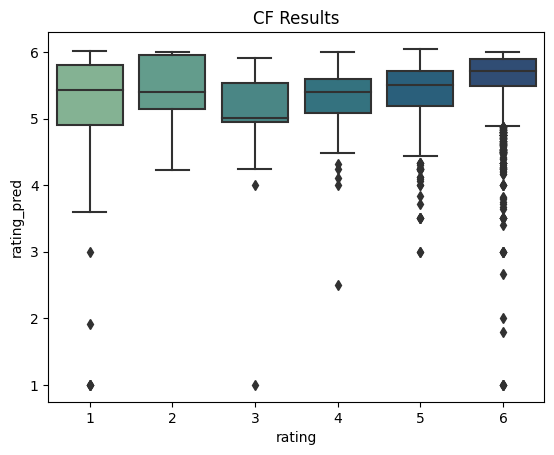
\includegraphics[width=0.6\textwidth]{CF.png}
    \caption{Distribution of predicted ratings across true ratings for CF Algorithm}
    \label{fig:CF}
\end{figure}

\subsection{Matrix Factorization CF}

I chose to perform the factorization into 40 latent factors because this number is a common default for recommendation packages in python. I decided to go with this approach rather choosing this number through cross-validation because I wanted to focus my time for this project more on exploring different algorithms rather than tuning this particular approach.  I initialized the $P$ and $Q$ matrices as uniform random matrices between 0 and 1. The shapes of these matrices are:

\begin{itemize}
    \item $P$: number of users by number of features (40).
    \item $Q$: number of features (40) by number of recipes.  
\end{itemize}

I trained the model by performing Gradient Descent for 100 iterations according to the matrix updates in section 4.4. Below is the training loss across iterations and the distribution of testing predictions versus true ratings. 

\begin{figure}[H]
    \centering
    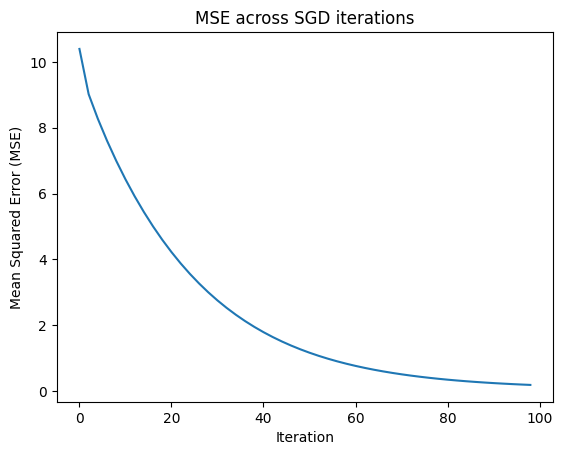
\includegraphics[width=0.45\textwidth]{MF_loss.png}
    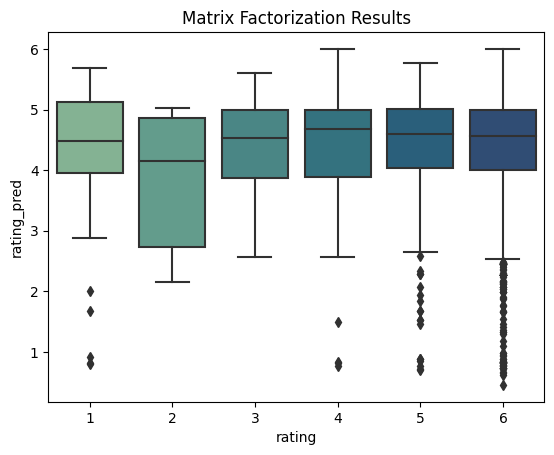
\includegraphics[width=0.45\textwidth]{MF.png}
    \caption{Left: MSE plotted across iterations, which shows the algorithm converging; Right: Distribution of predicted ratings across true ratings for Matrix Factorization Algorithm}
    \label{fig:CF}
\end{figure}

\subsection{CB model}

This model had the lowest coverage ratio of about 33\%. This means that this approach was able to generate predictions for only about one-third of the user-recipe pairs in the test data. This is because in order to generate a rating, the user must have rated another recipe that has at least one of the ingredients in the new recipe, which is a tall order for such a sparse data set. Overall, this approach did not perform as well as the CF approach in multiple ways. We can see as well in the plot below that there are similar issues of predicting mostly ratings between 5 and 6 across the whole data set. 


\begin{figure}[H]
    \centering
    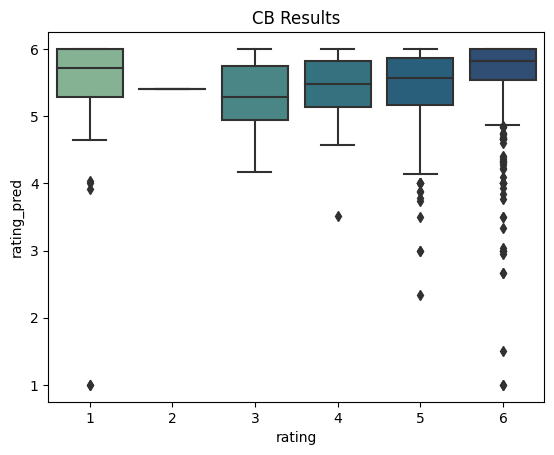
\includegraphics[width=0.6\textwidth]{CB.png}
    \caption{Distribution of predicted ratings across true ratings for CB Algorithm}
    \label{fig:CB}
\end{figure}

\subsection{Content-augmented CF}

For this approach, I used 50 most similar users as I did for the vanilla CF. 

Here, we again face the issue of there being very little variation in the predictions across all the true ratings. Unfortunately it appears that the main effect of including recipe-content information in the CF approach had the effect of bringing down the average rating by about 0.5 without doing much else. My guess as to why this is happening is that in this sparse data set, most users may have only rated a couple of recipes and therefore very little in that user across recipes. Extending the rating of this recipe to it's content data would not actually give a more varied look at the user's preferences, and might have teh effect of diluting the variation in the data set more by increasing the number of observations with the same associated rating. 
\begin{figure}[H]
    \centering
    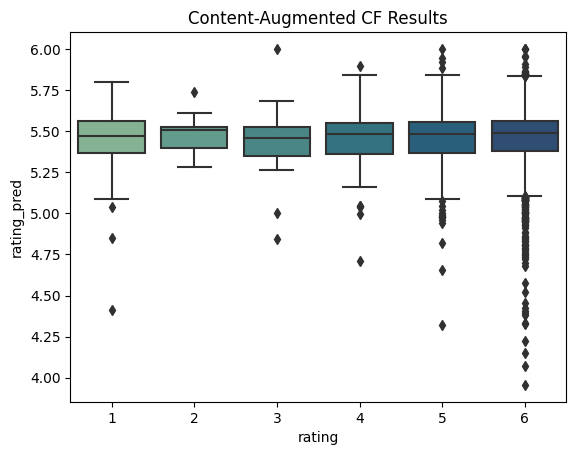
\includegraphics[width=0.6\textwidth]{CA_CF.png}
    \caption{Distribution of predicted ratings across true ratings for Content Augmented CF Algorithm}
    \label{fig:ratings_dist}
\end{figure}

\subsection{Content-augmented Matrix Factorization}

I started this process by creating the recipe-content matrix $X$, which is described in section 4.4. As with previous factorization approach, I chose to use 40 latent factors. I performed the optimization for this problem via Pytorch.  I initiated the matrices $P$ and $\Phi$ as random uniform distributions betwen 0 and 1. The three matrices had the following shapes:
\begin{itemize}
    \item $P$: number of users by number of features (40).
    \item  $\Phi$: number of features (40) by number of recipe contents.  
    \item $X$: number of recipe contents by number of recipes. 
\end{itemize}

I used Pytorch's typical workflow to calculate MSE loss and update the $P$ and $\Phi$ matrices via Gradient Descent on each training iteration. I trained for 500 iterations. Below is the training loss across iterations and the distribution of testing predictions versus true ratings. 

\begin{figure}[H]
    \centering
    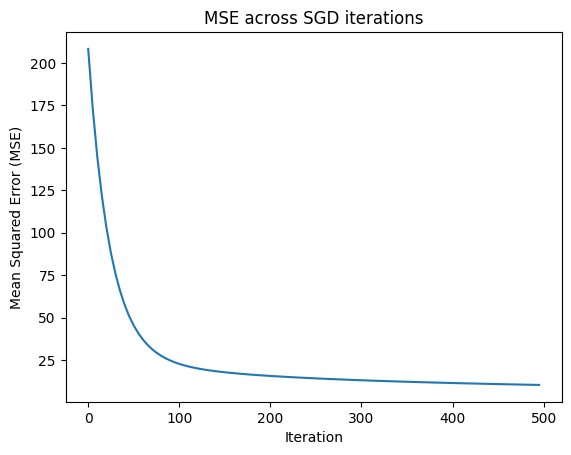
\includegraphics[width=0.45\textwidth]{MF_hybrid_loss.png}
    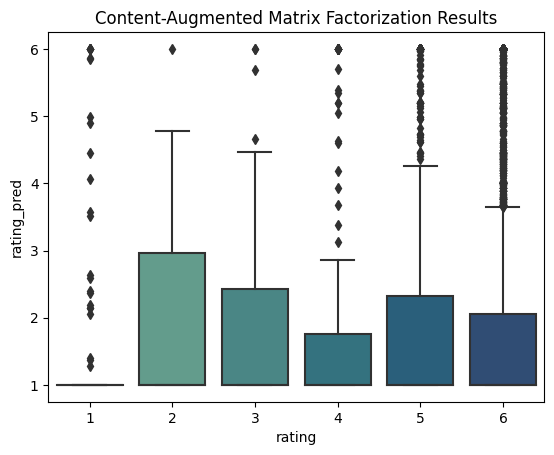
\includegraphics[width=0.45\textwidth]{MF_hybrid.png}
    \caption{Left: MSE plotted across iterations, which shows the algorithm converging; Right: Distribution of predicted ratings across true ratings for Matrix Factorization Algorithm}
    \label{fig:CF}
\end{figure}

\subsection{Summary, Future Directions}

In conclusion, I did not find that including content-related recipe such as ingredients, flavors, and cooking techniques universally improved the quality of user-recipe pair rating predictions. Overall, the best performance was actually found from vanilla CF, despite the fact that matrix factorization is commonly considered to be the most performant CF approach. I imagine that if I had the computational resources to train a matrix factorization model for longer and perform a complete hyperparameter tuning, I would get better results for that model. Compared to pure CB, CF approach did result in more accurate predictions, and combining content with vanilla CF improved the metrics in comparison with pure CB. 

For future experimentation, I would want to investigate the extent of overlap of recipe content (ingredients, etc.) across recipes. It's possible that if there is a large amount of overlap, the result of including more content data is actually diluting the personalized information in the data set. An additional avenue for experimentation is the distribution of ratings in the training data. While I'm sure that this skewed distribution had some effect on the performance of these algorithms, re-sampling the data so that the ratings were normally or uniformly distributed would result in a data set that is not representative of real-world rating systems where these algorithms would be implemented. When it comes to including content-based information in CF recommendation algorithms, the challenge is include enough information to augment, but not too much to decrease the variation across items or users. Therefore, in the future I would want to try a tuning paradigm where different amounts of content information is included and  the quality of predictions as well as parameters of the training data distribution are compared. 

\newpage

\section{References}
\begin{enumerate}
    \item Trang Tran, T. N., Atas, M., Felfernig, A., & Stettinger, M. (2018). An overview of recommender systems in the healthy food domain. \textit{Journal of Intelligent Information Systems}, 50 (pp. 501-526).
    \item Pecune, F., Callebert, L., & Marsella, S. (2020, September). A Recommender System for Healthy and Personalized Recipes Recommendations. In \textit{HealthRecSys@ RecSys} (pp. 15-20).
    \item Van Pinxteren, Y., Geleijnse, G., & Kamsteeg, P. (2011, February). Deriving a recipe similarity measure for recommending healthful meals. In \textit{Proceedings of the 16th international conference on Intelligent user interfaces} (pp. 105-114).
    \item Masthoff, J. (2011). Group recommender systems: Combining individual models. \textit{Recommender systems handbook}, Springer (pp. 677–702).
    \item Ajitsaria, A. Build a Recommendation Enging with Collaborate Filtering. \textit{RealPython.com}
    \item Freyne, J., & Berkovsky, S. (2010, February). Intelligent food planning: personalized recipe recommendation. In \textit{Proceedings of the 15th international conference on Intelligent user interfaces} (pp. 321-324).
    \item Burke, R. (2002). Hybrid Recommender Systems: Survey and Experiments. \textit{User Model User-Adap Inter} 12, (pp. 331–370).
    \item Aberg, J. (2006, January). Dealing with Malnutrition: A Meal Planning System for Elderly. In 
    \textit{AAAI spring symposium: argumentation for consumers of healthcare} (pp. 1-7).
    \item Luo, S. (2018, December). Introduction to Recommender System Approaches of Collaborative Filtering: Nearest Neighborhood and Matrix Factorization. \textit{towardsdatascience.com}
    \item Forbes, P., & Zhu, M. (2011, October). Content-boosted matrix factorization for recommender systems: experiments with recipe recommendation. In \textit{Proceedings of the fifth ACM conference on Recommender systems} (pp. 261-264).
    \item X. Luo, M. Zhou, Y. Xia and Q. Zhu. (May 2014). An Efficient Non-Negative Matrix-Factorization-Based Approach to Collaborative Filtering for Recommender Systems," in \textit{IEEE Transactions on Industrial Informatics,} vol. 10, no. 2 (pp. 1273-1284)
\end{enumerate}


\end{document}
